\documentclass[a4paper,12pt]{article}

\usepackage[pdftex]{graphicx}

\newcommand{\menu}[2]{{\it \vskip2mm #1 $\rightarrow$ #2 \vskip2mm}}
\newcommand{\dynmenu}[3]{{\it \vskip2mm #1 $\rightarrow$ #2 $\rightarrow$ #3 \vskip2mm}}

\title{ElmerGUI manual}
\author{Mikko Lyly}

\begin{document}
\maketitle

\newpage

\tableofcontents

\newpage

\section{Introduction}

ElmerGUI is a graphical user interface for the Elmer software suite
\cite{ElmerHome}. The program is capable of importing finite element mesh files in
various formats, generating finite element partitionings for models with piecewise linear
boundaries, setting up PDE-systems to solve, and exporting model data and result files
for ElmerSolver and ElmerPost.

\begin{figure}[ht]
\begin{center}
 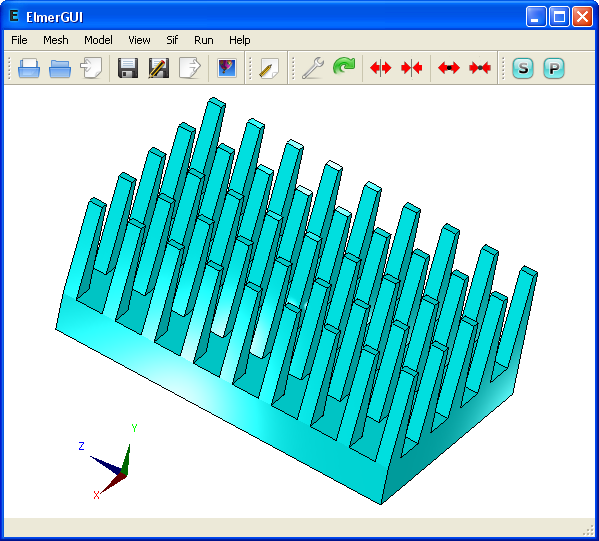
\includegraphics[scale=0.5]{images/elmergui.png}
\caption{Main window of ElmerGUI.}
\end{center}
\end{figure}

ElmerGUI has been written to facilitate the usage of ElmerSolver. It provides interfaces
to the most common solver modules (such as heat transfer, linear elasticity, and
Navier-Stokes equations) and to some generic numerical methods (such as iterative solvers
and ILU preconditioners), but it is far from complete in what comes to the full potential
of the solver. The best and most accurate control over ElmerSolver is still obtained
by direct modification of the solver input files according to the reference manuals.

One of the main features of ElmerGUI is the interface to the parallel version of the
solver, i.e., ElmerSolver\_mpi. The GUI hides from the user a number of operations that
are normally performed from command line with various external tools (domain
decomposition, launching the MPI-processes, and merging the results). The user is only
expected to prescribe the number of processes and the rest is transparent. This makes
it possible to use Elmer with multi-core processors even on an interactive desktop environment.

The menus of ElmerGUI are programmable and it should be relatively easy to strip and
customize the interface for any specific application. An example of customizing the
menus is provided in appendix A. 

ElmerGUI relies on the Qt4 cross platform framework \cite{QtHome} and it uses the Qwt5 libray \cite{QwtHome} for technical applications. The program is capable of linking against certain external finite element and cad libraries, such as libtet \cite{TetgenHome} and libng \cite{NetgenHome}. If you are planning to use libtet as a module with ElmerGUI, please consult the web site of Tetgen for licensing.

\section{Installation from source}

The source code of ElmerGUI is available at the subversion repository of SourceForge.Net. The GPL licenced source may be downloaded by executing the following command with a SVN client program (on Windows the Tortoise SVN client is recommended):

\begin{footnotesize}
\begin{verbatim}
svn co https://elmerfem.svn.sourceforge.net/svnroot/elmerfem/trunk trunk
\end{verbatim}
\end{footnotesize}
\noindent This will retrieve the current development version of the whole Elmer-suite.

\subsection{Linux}

Make sure that you have the development packages of Qt4 and Qwt5 installed on your system (i.e., libraries, headers, and program development tools). Qt version 4.2 or higher is recommended.

Execute the following sequence of commands in a terminal window:
\begin{verbatim}
$ cd elmerfem/trunk/misc/Mesh3D
$ qmake Mesh3D_Linux.pro
$ make
$ mv ./Mesh3D ./ElmerGUI
\end{verbatim}
It is possible that the project file ``Mesh3D\_Linux.pro'' needs to be edited depending on how and where Qwt5 has been installed.

Finally, set up the environment variable {\tt ELMERGUI\_HOME}, add it to {\tt PATH}, and copy the file ``ElmerGUI'' as well as the directory ``edf'' in this location:
\begin{verbatim}
$ export ELMERGUI_HOME=$ELMER_HOME/bin
$ export PATH=$PATH:$ELMERGUI_HOME
$ cp -r ./ElmerGUI ./edf $ELMERGUI_HOME
\end{verbatim}

\subsection{Windows}

The installation instructions for Windows are almost the same as for Linux. You will need  MinGW and MSYS and the open source version of Qt4 installed on your system \cite{QtHome}.  Qwt5 has to be compiled from source \cite{QwtHome}.

Once the prequisites are fulfilled, execute the following sequence of command in a MSYS shell:
\begin{verbatim}
$ cd elmerfem/trunk/misc/Mesh3D
$ qmake Mesh3D_MinGW.pro
$ make
$ mv ./release/Mesh3D.exe ./ElmerGUI.exe
\end{verbatim}
It is possible that the project file ``Mesh3D\_MinGW.pro'' needs to be edited depending on how and where Qwt5 has been installed.

Finally, set up the environment variable {\tt ELMERGUI\_HOME}, add it to {\tt PATH}, and copy the executable ``ElmerGUI.exe'' and the directory ``edf'' into this location:
\begin{verbatim}
$ export ELMERGUI_HOME=$ELMER_HOME/bin
$ export PATH=$PATH:$ELMERGUI_HOME
$ cp -r ./ElmerGUI.exe ./edf $ELMERGUI_HOME
\end{verbatim}

\section{Input files}

\subsection{Geometry input files and mesh generation}

ElmerGUI is capable of importing finite element mesh files and generating two or three
dimensional finite element partitionings for bounded domains with piecewise linear
boundaries. It is possible to use one of the following mesh generators:
\begin{itemize}
 \item ElmerGrid (built-in)
 \item Tetgen (optional)
 \item Netgen (optional)
\end{itemize}
The default import filter and mesh generator is ElmerGrid. Tetgen and Netgen are optional
modules, which may or may not be available.

An import filter or a mesh generator is selected automatically by ElmerGUI when a geometry
input file is opened from the File menu:

\menu{File}{Open...}

The selection is based on the input file suffix according to Table 1. If two or more
generators are capable of handing the same format, then the user defined ``preferred
generator'' will be used. The preferred generator is defined in

\menu{Mesh}{Configure...}

\begin{center}
\begin{tabular}{|c|c|c|c|}
\hline
 Suffix & ElmerGrid & Tetgen & Netgen \\
\hline 
.FDNEUT & yes & no & no \\
.grd  & yes & no & no \\
.msh & yes & no & no \\
.mphtxt & yes & no & no \\
.off & no & yes & no \\
.ply & no & yes & no \\
.poly & no & yes & no \\
.smesh & no & yes & no \\
.stl  & no & yes & yes \\
.unv & no & yes & no \\
\hline
\end{tabular}
\vskip5mm
Table 1. Input files and capabilities of the mesh generators.
\end{center}

Once the input file has been opened, it is possible to modify the mesh parameters
and remesh the geometry. The mesh parameters can be found from the same place as the preferred generator. The control string for Tetgen has been discussed and explained in detail in \cite{TetgenHome}.

The mesh generator is reactivated from the Mesh menu by choosing

\menu{Mesh}{Remesh}
\noindent In case of problems, the meshing thread may be terminated from
\menu{Mesh}{Terminate}

\subsection{Elmer mesh files}

An Elmer mesh consists of the following four text files (detailed description of the file format can be found from Appendix B):

\begin{verbatim}
mesh.header 
mesh.nodes 
mesh.elements 
mesh.boundary 
\end{verbatim}


\noindent The files have to be located side by side in the same mesh directory.

Elmer mesh files may be loaded and/or saved by opening the mesh directory fro the File menu:
\menu{File}{Load mesh...}
\noindent and/or
\menu{File}{Save as...}

\subsection{Project files}

An ElmerGUI project consists of a project directory with Elmer mesh files and a set of
.dat files defining the contents of the menus. Projects may be loaded and/or saved from
the File menu as
\menu{File}{Load project...}
\noindent and/or
\menu{File}{Save project...}

When an ElmerGUI project is loaded, a new solver input file will be generated and saved
in the project directory using the sif-name defined in
\menu{Model}{Setup...}
\noindent If there is an old solver input file with the same name, it will be overwritten.

The contents of a typical project directory is the following:

\begin{verbatim}
bodyforce.dat 
bodyproperty.dat 
boundarycondition.dat 
boundaryproperty.dat 
case.sif 
ELMERSOLVER_STARTINFO 
equation.dat 
initialcondition.dat 
material.dat 
mesh.boundary 
mesh.elements 
mesh.header 
mesh.nodes
\end{verbatim}

\section{Model definitions}

\subsection{Setup menu}

The general setup menu can be found from
\menu{Model}{Setup...}
\noindent This menu defines the basic variables for the ``Header'', ``Simulation'',
and ``Constants'' blocks for a solver input file. The contents of these blocks have
been discussed in detail in the SolverManual of Elmer \cite{ElmerHome}.

\begin{figure}[ht]
\begin{center}
 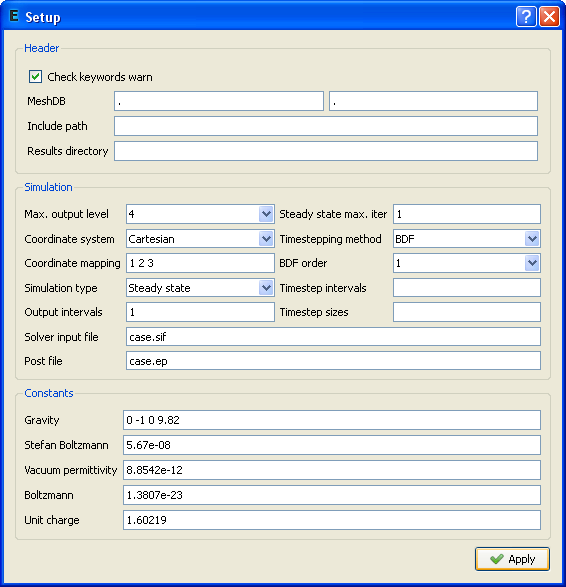
\includegraphics[scale=0.5]{images/setupmenu.png}
\caption{Setup menu.}
\end{center}
\end{figure}

\subsection{Equation menu}

The first ``dynamical menu'' constructed from the ElmerGUI definition files (see Appendix A) is
\menu{Model}{Equation}
\noindent This menu defines the PDE-system to be solved as well as the numerical
methods and parameters used in the solution. It will be used to generate the ``Solver''
blocks in a solver input file.

A PDE-system (a.k.a ``Equation'') is defined by choosing
\dynmenu{Model}{Equation}{Add...}

\begin{figure}[ht]
\begin{center}
 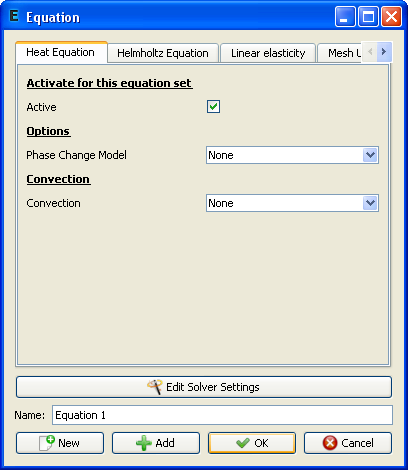
\includegraphics[scale=0.5]{images/equation.png}
\caption{Equation menu.}
\end{center}
\end{figure}

Go through the tabs and check the ``Active'' boxes of all individual equations that
constitute your model. The numerical methods and parameters can be
selected and tuned by pressing the ``Edit Solver Settings'' button. Finally, name the
PDE-system in the ``Name'' line edit box, and apply the system to a set of bodies.
Once the PDE-system has been defined, press the Ok-button. The equation remains
visible and editable under the Model menu.


\begin{figure}[ht]
\begin{center}
 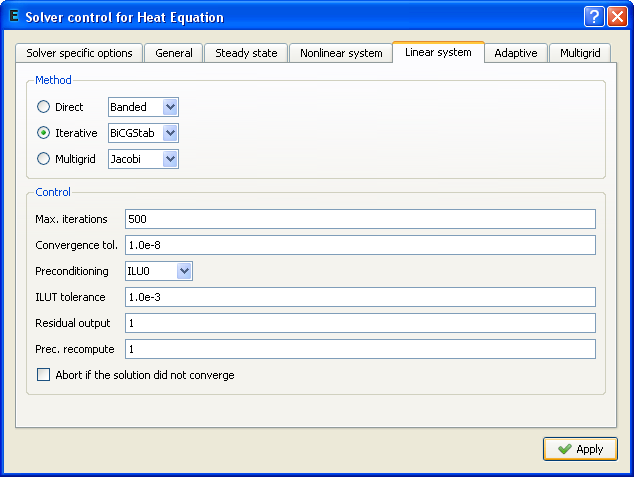
\includegraphics[scale=0.5]{images/solversettings.png}
\caption{Solver settings menu.}
\end{center}
\end{figure}

{\bf Tip}: It is possible to attach an equation to a body by holding down the SHIFT-key
while double clicking one of its surfaces. A pop up menu will then appear,
listing all possible attributes that can be attached to the selection. Choose the
attributes and press Ok.

\begin{figure}[ht]
\begin{center}
 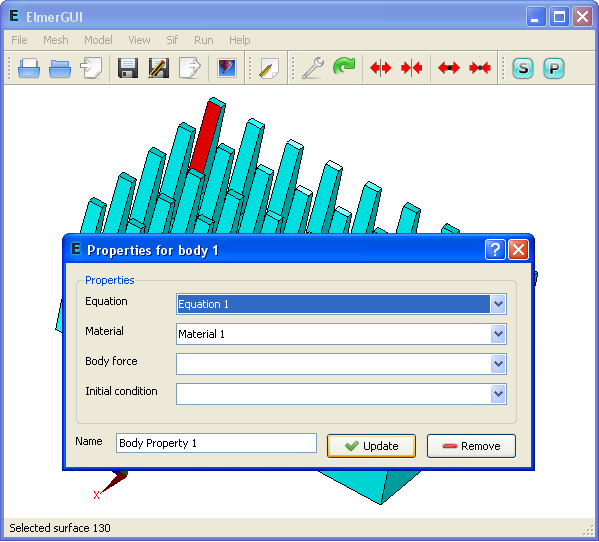
\includegraphics[scale=0.5]{images/bodyproperties.png}
\caption{Body property editor is activated by holding down the SHIFT key while double
clicking a surface.}
\end{center}
\end{figure}

\subsection{Material menu}

The next menu is related to material and model parameters:
\menu{Model}{Material}
\noindent This menu will be used to generate the ``Material'' blocks in a solver
input file.

In order to define a material parameter set and attach it to bodies, choose
\dynmenu{Model}{Material}{Add...}
\noindent 

\begin{figure}[ht]
\begin{center}
 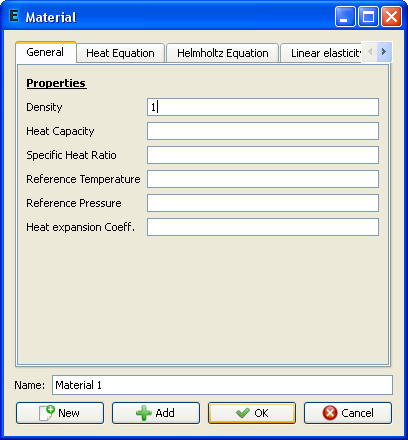
\includegraphics[scale=0.5]{images/material.png}
\caption{Material menu.}
\end{center}
\end{figure}

Again, it is possible to attach the material to a body also by holding down the SHIFT-key while double clicking one of its boundaries.

\vskip2mm

{\bf Note}: The value of density should always be defined in the ``General'' tab. This
field should never be left undefined.

\vskip2mm

{\bf Tip}: If you set focus in a line edit box of a dynamical menu and press Enter, a small
text edit dialog will pop up. This allows the input of more complicated expressions
than just constants. As an example, go to {\it Model $\rightarrow$ Material} and choose
{\it Add...} Place the cursor in the ``Heat conductivity'' line edit box of ``Heat
equation'' and press Enter. You can then define the heat conductivity
as a function of temperature as a piecewise linear function. An example is show in
Figure N. In this case, the heat conductivity gets value 10 if the temperature is less
than 273 degrees. It then rises from 10 to 20 between 273 and 373 degrees, and
remains constant 20 above 373 degrees.

\begin{figure}[ht]
\begin{center}
 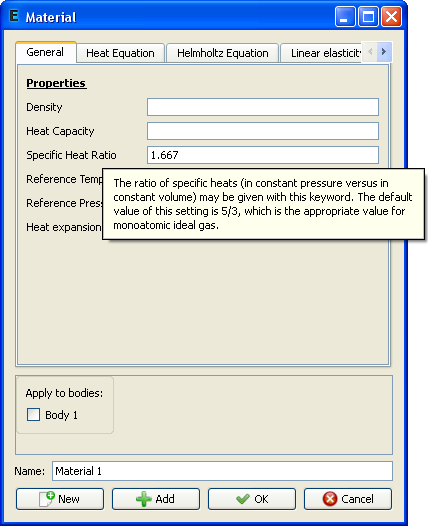
\includegraphics[scale=0.5]{images/tooltip.png}
\caption{Tooltips are shown by holding down the SHIFT and F1 keys.}
\end{center}
\end{figure}

{\bf Tip}: If the user presses SHIFT and F1, a tooltip for the active widget will be displayed.

\begin{figure}[ht]
\begin{center}
 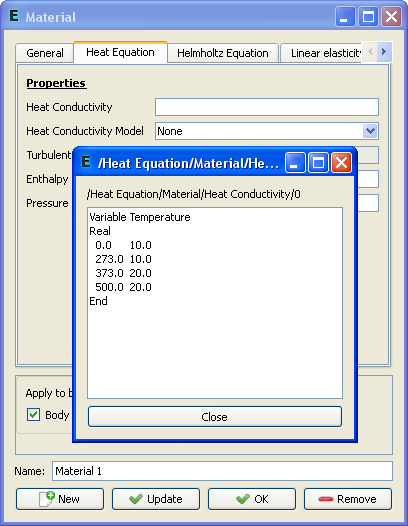
\includegraphics[scale=0.5]{images/textedit.png}
\caption{Text edit extension of a line edit box is activated by pressing Enter.}
\end{center}
\end{figure}

\subsection{Body force menu}

The next menu in the list is
\menu{Model}{Body force}
\noindent This menu is used to construct the ``Body force'' blocks in a
solver input file.

Again, choose
\dynmenu{Model}{Body force}{Add...}
\noindent to define a set of body forces and attach it to the bodies.

\begin{figure}[ht]
\begin{center}
 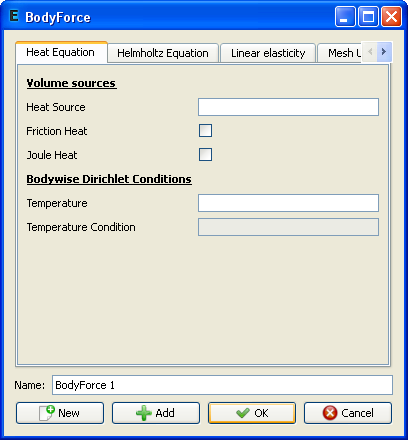
\includegraphics[scale=0.5]{images/bodyforce.png}
\caption{Body force menu.}
\end{center}
\end{figure}

\subsection{Initial condition menu}

The last menu related to body properties is
\menu{Model}{Initial condition}
\noindent 
Once again, choose
\dynmenu{Model}{Initial condition}{Add...}
\noindent to define a set of initial conditions and attach it to the bodies.

This menu is used to construct the ``Initial condition'' blocks in a
solver input file.

\begin{figure}[ht]
\begin{center}
 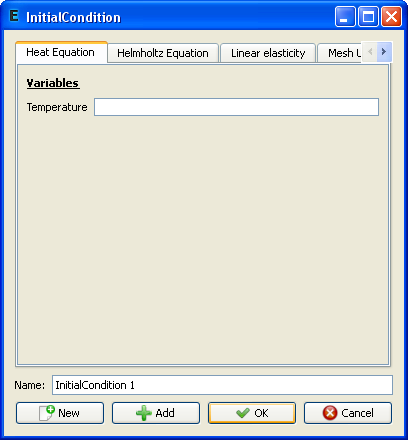
\includegraphics[scale=0.5]{images/initialcondition.png}
\caption{Initial condition menu.}
\end{center}
\end{figure}

\subsection{Boundary condition menu}

Next, there is a menu related to surfaces and edges:
\menu{Model}{Boundary condition}
\noindent This menu is used to construct the ``Boundary condition'' blocks in a
solver input file.

Choose
\dynmenu{Model}{Boundary condition}{Add...}
\noindent to define a set of boundary conditions and attach it to the boundaries.

\begin{figure}[ht]
\begin{center}
 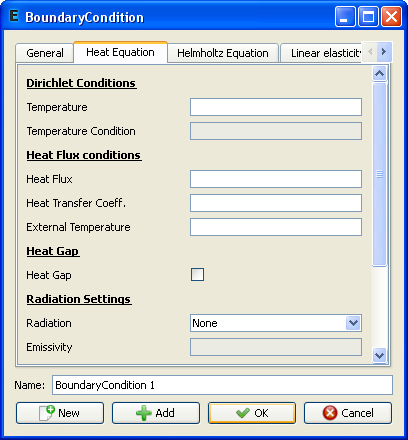
\includegraphics[scale=0.5]{images/boundarycondition.png}
\caption{Boundary condition menu.}
\end{center}
\end{figure}

{\bf Tip}: It is possible to attach a boundary condition to a boundary by holding down 
the ALT or ALTGR-key while double clicking a surface or edge. A pop up menu will appear, listing all possible conditions that can be attached to the selection. 
Choose a condition from the combo box and finally press Ok.

\begin{figure}[ht]
\begin{center}
 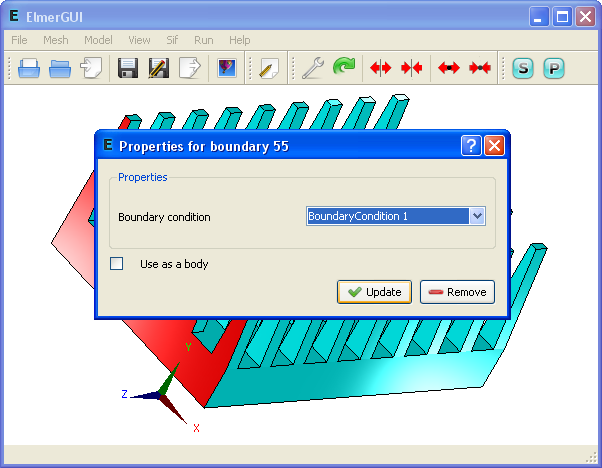
\includegraphics[scale=0.5]{images/boundaryproperties.png}
\caption{Boundary property editor activated by holding down the ALTGR key while double
clicking a surface.}
\end{center}
\end{figure}

\section{Utility functions}

\subsection{Boundary division and unification}

Some of the input file formats listed in Table 1 are not necessarily best suited for
FE-calculations. The .stl format (stereo litography format), for example, is unable
to distinguish between different boundary parts with different attributes. Moreover, it
approximates the boundary by disconnected triangles. The file format would
be rather useless in this context, unless there were other ways to identify the
boundary parts and methods for dealing with the possible discontinuities.

ElmerGUI provides a minimal set of tools for boundary division and unification. The
division is based on ``sharp edge detection''. An edge between two boundary elements
is considered sharp, if the angle between the normals exceeds a certain value (20
degrees by default). The sharp edges are then used as a mortar to divide the surface
into parts. The user may perform a sharp edge detection and boundary division from
the Mesh menu by choosing
\menu{Mesh}{Divide surface...}
\noindent In 2D the corresponding operation is
\menu{Mesh}{Divide edge...}
\noindent The resulting parts are enumerated starting from the first free index.

Sometimes, the above process produces too many distinct parts, which eventually need to
be (re)unified. This can be done by selecting a group of surfaces by holding down the
CTRL-key while double clicking the surfaces and choosing
\menu{Mesh}{Unify surface...}
\noindent The same operation in 2D is
\menu{Mesh}{Unify edge...}
\noindent The result will inherit the smallest index from the selected group.

The sharp edges that do not belong to a closed loop may be removed by
\menu{Mesh}{Clean up}
\noindent This operation has no effect on the boundary division, but sometimes it makes
the result look better.

\subsection{Saving pictures}

The model drawn on the display area may be scanned into a 24-bit RGB image and saved in
several picture file formats:
\menu{File}{Save picture as...}
\noindent The function supports .bmp, .jpg, .png, .pbm, .pgm, and .ppm file extensions.

\subsection{View menu}

The View menu provides several utility functions for controlling the visual behaviour
of ElmerGUI. The function names should be more or less self explanatory.

\section{Solver input files}

The contents of the Model menu are passed to the solver in the form of a solver
input file. A solver input file is generated by choosing
\menu{Sif}{Generate}
\noindent The contents of the file are editable:
\menu{Sif}{Edit...}

The new sif file needs to saved before it becomes active. The recommended
method is
\menu{File}{Save project...}
\noindent In this way, also the current mesh and project files get saved in the
same directory, avoiding possible inconsistencies later on.

\section{Solution and post processing}

\subsection{Running the solver}

Once the solver input file has been generated and the project has been saved,
it is possible to actualy solve the problem:
\menu{Run}{Run solver}
\noindent This will launch either a single process for ElmerSolver (scalar solution)
or multiple MPI-processes for ElmerSolver\_mpi (parallel solution) depending on the
definitions in
\menu{Run}{Parallel settings...}

\begin{figure}[ht]
\begin{center}
 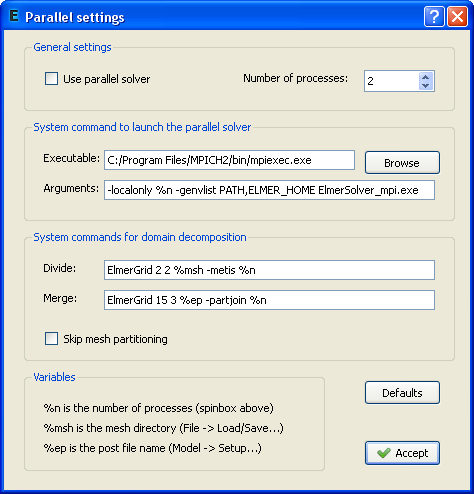
\includegraphics[scale=0.5]{images/parallelsettings.png}
\caption{Parallel settings dialog.}
\end{center}
\end{figure}

The parallel menu has three group boxes. Usually, the user is supposed to touch
only the ``General settings'' group and select the number of processes to execute.
The two remaining groups deal with system commands to launch MPI-processes and
external tools for domain decomposition.  The parallel menu is greyed out if
ElmerSolver\_mpi is not present at start-up.

When the solver is running, there is a log window and a convergence monitor
from which the iteration may be followed. In case of divergence or other troubles,
the solver may be terminated by choosing
\menu{Run}{Kill solver}

The solver will finally write a result file for ElmerPost in the project directory.
The name of the ep-file is defined in
\menu{Model}{Setup...}

\subsection{Post preocessor}

The post processor is activated from
\menu{Run}{Run postprocessor}
\noindent This will launch ElmerPost, which will read in the results and displays
a contour plot representing the solution. If the results were prodoced by the parallel solver, the domain decomposition used in the calculations will be shown.


\bibliographystyle{plain}
\bibliography{elmergui}

\appendix

\section{ElmerGUI definition files}

The directory {\tt ELMERGUI\_HOME} contains a subdirectory called ``edf''. This is the place where all ElmerGUI definition files (ed-files) reside. The definition files are XML-formatted text files which define the contents and appearance of the Model menu.

The ed-files are loaded iteratively from the edf-directory once and for all when ElmerGUI starts. Later, it is possible to view and edit their contents by choosing
\menu{File}{Definitions...}

\newpage

An ed-file has the following structure:
\begin{footnotesize}
\begin{verbatim}
<?xml version='1.0' encoding='UTF-8'?>
<!DOCTYPE edf>
<edf version="1.0">
   [PDE block]
   [PDE block]
   ...
   [PDE block]
</edf>
\end{verbatim}
\end{footnotesize}

The structure of a [PDE block] is the following:
\begin{footnotesize}
\begin{verbatim}
<PDE Name="My equation">
   <Name>
      My equation
   </Name>
   ...
   <Equation>
      [Widget block]
   </Equation>
   ...
   <Material>
      [Widget block]
   </Material>
   ...
   <BodyForce>
      [Widget block]
   <BodyForce>
   ...
   <InitialCondition>
      [Widget block]
   </InitialCondition>
   ...
   <BoundaryCondition>
      [Widget block]
   </BoundaryCondition>
</PDE>
\end{verbatim}
\end{footnotesize}
Note that the name of the PDE is defined redundantly in two occurances.

The basic stucture of a [Widget block] is the following:
\begin{footnotesize}
\begin{verbatim}
<Parameter Widget="Label">
   <Name> My label </Name>
</Parameter>
...
<Parameter Widget="Edit"> 
   <Name> My edit box </Name>
   <Type> Integer </Type>
   <Whatis> Meaning of my edit box </Whatis>
</Parameter>
...
<Parameter Widget="CheckBox">
   <Name> My check box </Name>
   <Type> Logical </Type>
   <Whatis> Meaning of my check box </Whatis>
</Parameter>
...
<Parameter Widget="Combo"> 
   <Name> My combo box </Name> 
   <Type> String </Type>
   <Item> <Name> My 1st item </Name> </Item>
   <Item> <Name> My 2nd item </Name> </Item>
   <Item> <Name> My 3rd item </Name> </Item>
   <Whatis> Meaning of my combo box </Whatis>
</Parameter>
\end{verbatim}
\end{footnotesize}

There are four types of widgets available:
\begin{itemize}
 \item Label (informative text)
 \item CheckBox (switches)
 \item ComboBox (selection from list)
 \item LineEdit (generic variables)
\end{itemize}
Each widget must be given a name and and a variable type: logical, integer, real, or  string. It is also a good practice to equip the widgets with tooltips explaining their purpose and meaning as clearly as possible.

Below is a working example of a minimal ElmerGUI definition file. It will add ``My equation'' to the equation tabs in the Model menu, see Figure N. The file is called ``sample.edf'' and it should be placed in {\tt ELMERGUI\_HOME/edf}.

\begin{footnotesize}
\begin{verbatim}
<?xml version='1.0' encoding='UTF-8'?>
<!DOCTYPE edf>
<edf version="1.0">
  <PDE Name="My equation">
    <Name> My equation </Name>
    <Equation>
      <Parameter Widget="Label">
        <Name> My label </Name>
      </Parameter>
      <Parameter Widget="Edit">
        <Name> My edit box </Name>
        <Type> Integer </Type>
        <Whatis> Meaning of my edit box </Whatis>
      </Parameter>
      <Parameter Widget="CheckBox">
        <Name> My check box </Name>
        <Type> Logical </Type>
        <Whatis> Meaning of my check box </Whatis>	  
      </Parameter>
      <Parameter Widget="Combo">
        <Name> My combo box </Name>
        <Type> String </Type>
        <Item> <Name> My 1st item </Name> </Item>
        <Item> <Name> My 2nd item </Name> </Item>
        <Item> <Name> My 3rd item </Name> </Item>
        <Whatis> Meaning of my combo box </Whatis>	  
      </Parameter>
    </Equation>
  </PDE>
</edf>
\end{verbatim}
\end{footnotesize}

\begin{figure}[ht]
\begin{center}
 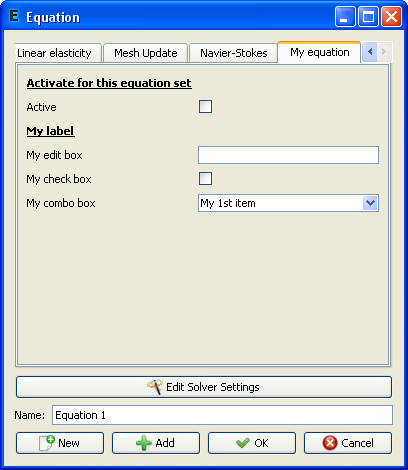
\includegraphics[scale=0.5]{images/edfsample.png}
\caption{Equation tab in Model menu produced by the sample ed-file.}
\end{center}
\end{figure}

More sophisticated examples with different tags and attribites can be found from the XML-files in  {\tt ELMERGUI\_HOME/edf}.

\newpage

\section{Elmer mesh files}

\noindent {\bf mesh.header}
\begin{verbatim}
nodes elements boundary-elements
types
type1 elements1
type2 elements2
...
typeN elementsN
\end{verbatim}

\vskip5mm

\noindent {\bf mesh.nodes}
\begin{verbatim}
node1 tag1 x1 y1 z1
node2 tag2 x2 y2 z2
...
nodeN tagN xN yN zN
\end{verbatim}

\vskip5mm

\noindent {\bf mesh.elements}
\begin{verbatim}
element1 body1 type1 n11 ... n1M
element2 body2 type2 n21 ... n2M
...
elementN bodyN typeN nN1 ... nNM
\end{verbatim}

\vskip5mm

\noindent {\bf mesh.boundary}
\begin{verbatim}
element1 boundary1 parent11 parent12 n11 ... n1M
element2 boundary2 parent21 parent22 n21 ... n2M
...
elementN boundaryN parentN1 parentN2 nN1 ... nNM
\end{verbatim}


\end{document}

